\documentclass[10pt,border=3mm,tikz]{standalone}
\usetikzlibrary{arrows.meta}
\usepackage{tkz-euclide}

\begin{document}
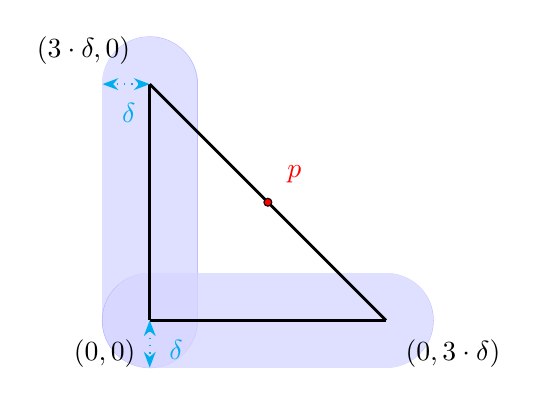
\begin{tikzpicture}[
    inner/.style={black,line width = 1pt,},
    outer/.style={double distance=12mm,
                  line cap=round,
                  blue!50,          % deal with overdrawings
                  opacity=.5,       % deal with overdrawings
                  line width=.2pt},
    > = {Stealth},                  % nicer arrow tip
    arr/.style={<->,cyan,dotted,line width=.6pt},
 ]

    \coordinate (A) at (0,0);
    \coordinate (B) at (3,0);
    \coordinate (C) at (0,3);
    \coordinate (D) at (1.5,1.5);

    \draw[outer] (A) to (C);
    \draw[outer] (A) to (B);

    \node[label = {[text = black]245:$(0,0)$}] at (A) {};
    \node[label = {[text = black]315:$(0,3\cdot\delta)$}] at (B) {};
    \node[label = {[text = black]135:$(3\cdot\delta,0)$}] at (C) {};

    \draw[inner] (A) to (B);
    \draw[inner] (B) to (C);
    \draw[inner] (C) to (A);

    \draw[fill = red] (D) circle (0.05);
    \node[label = {[text = red]45:$p$}] at (D) {};

    \draw[arr] (A) -- (0,-0.6);
    \draw[arr] (C) -- (-0.6,3);

    \node[label = {[text = cyan]245:$\delta$}] at (C) {};
    \node[label = {[text = cyan]315:$\delta$}] at (A) {};

 \end{tikzpicture}
\end{document}